\documentclass[a4paper]{article}

%%%%%%%%%%%%%%%%%%%%%%%
% gebruikte pakketten %
%%%%%%%%%%%%%%%%%%%%%%%

\usepackage[dutch]{babel}
\usepackage[utf8]{inputenc}
\usepackage{amsmath}
\usepackage{amsthm}
\usepackage{graphicx}
\usepackage[colorinlistoftodos]{todonotes}
\usepackage{subfig}
\usepackage{mdframed}
\usepackage{color}
\usepackage{microtype} 					% Meer esthetische spatiëring letters
\usepackage[utf8]{inputenc}
\usepackage[T1]{fontenc} 
\usepackage{enumerate}
\usepackage[shortlabels]{enumitem} 
\usepackage{multicol}
\usepackage{smartdiagram}
\usesmartdiagramlibrary{additions}
\setlist[enumerate]{topsep=0pt} 
\setlist[description]{topsep=0pt}
\setlist[itemize]{topsep=0pt}

%%%%%%%%%%%%%%%%%%%%%%%%%%%%%%%%%%%%%%%%%%
% definities van een nieuwe omgeving %
%%%%%%%%%%%%%%%%%%%%%%%%%%%%%%%%%%%%%%%%%% 

\newcounter{derive}
\setcounter{derive}{1}

\newenvironment{derive} [2]
	{\begin{mdframed} [linecolor=violet, linewidth=2, backgroundcolor=magenta!15, leftmargin=0.25cm, rightmargin=0.25cm]
    \noindent \textcolor{violet}{\textbf{Derivecode}} \textcolor {violet} {\arabic{derive}} \textcolor{violet}{\textrm{(#1)}}
    \newline \newline \noindent 	\textcolor{blue}
    {\textrm{#2}}
    \refstepcounter{derive}
    \end{mdframed}}


%%%%%%%%%%%%%%%%%%%%%%%%%%%%%%%%%%%
% een hele serie eigen definities %
%%%%%%%%%%%%%%%%%%%%%%%%%%%%%%%%%%%

\newcommand{\Z}{\mathbb{Z}}
\newcommand{\Zn}{\mathbb{Z}_n}
\newcommand{\N}{\mathbb{N}}
\newcommand{\Q}{\mathbb{Q}}
\newcommand{\R}{\mathbb{R}}
\newcommand{\C}{\mathbb{C}}
\def \Cscr{{\mathcal C}}
\def \Bscr{{\mathcal B}}
\def \Ascr{{\mathcal A}}
\def \Escr{{\mathcal E}}
\renewcommand{\Im}{\mathrm{Im}}
\newcommand{\voorbr}[1]{\langle #1\rangle}
\newcommand{\abs}[1]{\lvert #1\rvert}
\renewcommand{\vec}[1]{#1}
\newcommand{\p}[1]{\left( #1 \right)}
\newcommand{\pmM}[1]{\left(\begin{smallmatrix} #1 \end{smallmatrix}\right)}
\newcommand{\pmMr}[1]{\left(\begin{smallmatrix*}[r] #1 \end{smallmatrix*}\right)}
\newcommand{\pM}[1]{\left(\begin{matrix} #1 \end{matrix}\right)}
\newcommand{\pMr}[1]{\left(\begin{matrix*}[r] #1 \end{matrix*}\right)}
\newcommand{\dmM}[1]{\left|\begin{smallmatrix} #1 \end{smallmatrix}\right|}
\newcommand{\dmMr}[1]{\left|\begin{smallmatrix*}[r] #1 \end{smallmatrix*}\right|}
\newcommand{\dM}[1]{\left|\begin{matrix} #1 \end{matrix}\right|}
\newcommand{\dMr}[1]{\left|\begin{matrix*}[r] #1 \end{matrix*}\right|}

%%%%%%%%%%%
% kleuren %
%%%%%%%%%%%

\colorlet{steunkleur}{black}
\colorlet{steunkleurlicht}{steunkleur!30!white}
\colorlet{steunkleurkader}{steunkleur!7!white}

%%%%%%%%%%%%%%%%%%
% Kader-stijlen  %
%%%%%%%%%%%%%%%%%%

\mdfdefinestyle{kaderstijl_rand_licht}%
{skipabove=10pt,
skipbelow=1pt,
linecolor=steunkleurlicht,
linewidth=0.5pt,
%backgroundcolor=steunkleurkader,
innerleftmargin=5pt,
innerrightmargin=5pt,
innertopmargin=5pt,
leftmargin=0cm,
rightmargin=0cm,
innerbottommargin=5pt,
%needspace=30pt,
}

\mdfdefinestyle{kaderstijl_lrand}%
{skipabove=7pt,
skipbelow=0pt,
rightline=false,
leftline=true,
topline=false,
bottomline=false,
%backgroundcolor=steunkleurkader,
linecolor=steunkleurlicht,
innerleftmargin=5pt,
innerrightmargin=0pt,
innertopmargin=5pt,
innerbottommargin=3pt,
leftmargin=0cm,
rightmargin=0cm,
linewidth=3pt,
%needspace=30pt
}


%%%%%%%%%%%%%%%%%%%%%%%%%%%%%%
% Theorem-stijlen toekenning %
%%%%%%%%%%%%%%%%%%%%%%%%%%%%%%

\theoremstyle{plain}
\newtheorem{stelling}{\color{steunkleur}Stelling}
\newtheorem{eigenschap}[stelling]{\color{steunkleur}Eigenschap}
\newtheorem{propositie}[stelling]{\color{steunkleur}Propositie}
\newtheorem{lemma}[stelling]{\color{steunkleur}Lemma}
\newtheorem{vraag}[stelling]{\color{steunkleur}Vraag}
\newtheorem{gevolg}[stelling]{\color{steunkleur}Gevolg}

\theoremstyle{definition}
\newtheorem{definitie}[stelling]{\color{steunkleur}Definitie}
\newtheorem{definitie-propositie}[stelling]{\color{steunkleur}Definitie-Propositie}
\newtheorem{terminologie}[stelling]{\color{steunkleur}Terminologie}
\newtheorem{bewering}[stelling]{\color{steunkleur}Bewering}
\newtheorem{voorbeeld}[stelling]{\color{steunkleur}Voorbeeld}
\newtheorem{constructie}[stelling]{\color{steunkleur}Constructie}
\newtheorem*{algoritme}{\bfseries\color{steunkleur}ALGORITME}
\newtheorem {oef} {Oefening}
\newenvironment {enumoef} {\begin{enumerate}[\rm (a)]} {\end{enumerate}}
\newenvironment {enumstel} {\begin{enumerate}[\rm (i)]} {\end{enumerate}}

\theoremstyle{remark}
\newtheorem{opmerking}[stelling]{Opmerking}
\newtheorem*{opmerking*}{Opmerking}
\newtheorem{opdracht}[stelling]{Opdracht}
\newtheorem*{bewijstechniek}{\bfseries Bewijstechniek}
\newtheorem{opdracht_moeilijk}[stelling]{\bfseries *Opdracht}
\newtheorem{notatie}[stelling]{Notatie}
\newtheorem*{notatie*}{Notatie}

%%%%%%%%%%%%%%%%%%%%%
% Krijgen een kader %
%%%%%%%%%%%%%%%%%%%%%

\surroundwithmdframed[style=kaderstijl_vol_licht]{stelling}
\surroundwithmdframed[style=kaderstijl_vol_licht]{lemma}
\surroundwithmdframed[style=kaderstijl_vol_licht]{eigenschap}
\surroundwithmdframed[style=kaderstijl_vol_licht]{propositie}
\surroundwithmdframed[style=kaderstijl_vol_licht]{gevolg}
\surroundwithmdframed[style=kaderstijl_lrand]{opdracht}

\title{Handleiding voor RSA-krakers}
\author{Luc Van den Broeck}
\date{\today}

\begin{document}
\maketitle

\begin{abstract}
\noindent Achter de ontdekking van de RSA-codes zit heel wat mooie wiskunde, voornamelijk uit de getaltheorie. De wiskundige die onbewust hebben bijgedragen tot de ontdekking van de RSA-codes zijn Eratosthenes, Euclides, Fermat, Euler, Gauss, Bezout en Bachet. De wiskundigen die de RSA-codes bewust hebben ontdekt zijn Rivest, Shamir en Adleman. In deze cursus laten we zien welke bijdrage al deze wiskundigen hebben geleverd aan de codetheorie. We leggen eveneens uit hoe het RSA-codes-mechanisme werkt en hoe deze codes worden gekraakt. De softwarepakketten die hiervoor gebruikt worden zijn Derive (voor het didactische aspect) en Sage (voor de rekenkracht en voor het programmatorisch aspect)
\end{abstract}

\section{Een brokje geschiedenis}
Geen geheimcode ter wereld is zo vernuftig of ze wordt vroeg of laat ontraadseld. Het doorbreken van cryptografische barrières bij wijdvertakte computernetwerken heeft altijd al een bijzondere aantrekkingskracht uitgeoefend op gewiekste computeramateurs. Ook computeranalfabeten voelen vaak een heimelijke sympathie voor de jeugdige hackers die het avondjournaal halen door een geslaagde computerkraak. In dit seminarie kan je even proeven van de verboden vrucht van het codekraken \ldots tenminste indien je beschikt over het nodige geduld en over een voldoend snelle computer.

RSA-codes behoren tot de veiligste cryptografiesystemen ter wereld. Ze zijn in 1977 be-dacht door het drietal: Ronald Rivest, Adi Shamir en Leonard Adleman. Deze codes hebben een asymmetrisch sleutelmechanisme, d.w.z. dat de verzender en de ontvanger over een verschillende sleutel beschikken. RSA-codes hebben daarom de naam veilig maar omslachtig te zijn.

\begin{figure} [h]
\label{rivest}
\centering
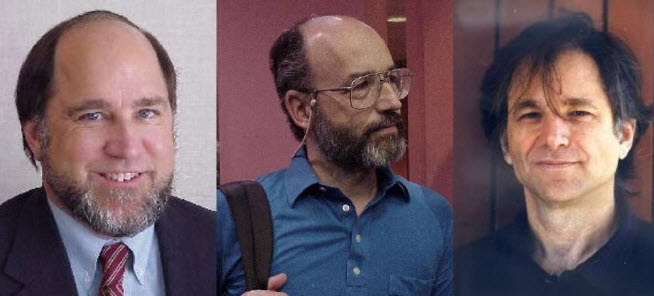
\includegraphics[width=\textwidth]{RivestShamirAdleman.jpg}
\caption{Ronald Rivest, Adi Shamir en Leonard Adleman}
\end{figure}

Rond dezelfde tijd werd in de Verenigde Staten een symmetrisch codesysteem met een snellere werking ontwikkeld: DES (Data Encryption System). Bij DES hebben de verzender en de ontvanger dezelfde sleutel, een bekritiseerbaar uitgangspunt. Om de veiligheid te garanderen stelt DES 72 biljard ($2^{56}$) verschillende geheime sleutels ter beschikking. DES wordt vaak gebruikt in de financiële wereld voor pinpasjes. Toen de bedenkers van de RSA-code de concurrentie van DES begonnen te voelen, loofden ze een prijs van 10000 \$ uit voor het kraken van een door DES gecodeerd bericht. Dit lukte pas in 1997.

Het vertrouwen in DES kreeg een deuk. Toevalligerwijze werd het jaar voordien een nieuw coderingssysteem ontwikkeld door de Vlamingen Vincent Rijmen (Leuven) en Johan Daemen (Achel). Het ‘Rijndaelsysteem’ oogstte wereldwijd bijval en werd in november 2001 door het Amerikaanse National Institute of Standards and Technology (NIST) uit 15 kandidaten verkozen tot Advanced Encryption Standard (AES). Momenteel is Vincent Rijmen docent op het departement van elektrotechniek aan de katholieke universiteit van Leuven. Joan Daemen doet onderzoek aan de Radboud Universiteit te Nijmegen.

Sinds het gebruik van het internet is de cryptografie  in een stroomversnelling geraakt. Een manier voor het coderen van mails is het softwarepakket Pretty Good Privacy (PGP), dat eveneens werkt met een asymmetrische versleuteling. PGP werd ontwikkeld door de Amerikaan Philip R. Zimmerman en werd in 1991 gratis aangeboden op het internetforum Usenet. De PGP-software maakt een toevallige sleutel aan op grond van de bewegingen van je muis. 

Codering van gegevens wordt ook gebruikt wanneer je veilige websites bezoekt, bijvoorbeeld om te internetbankieren. Je kunt deze sites herkennen aan het verschijnen van een hangslotsymbooltje rechtsonder in het scherm van de browser en ook aan het webadres dat begint met ‘https’ in plaats van ‘http’. Velige sites gebruiken een technologie die Secure Sockets Layer (SSL) heet. Ook SSL gebruikt een asymmetrische codering. 

De wiskundige achtergrond van de RSA-code is vrij eenvoudig. Deze code steunt op zes mijlpalen uit de getaltheorie: de priemgetallenzeef van Erathostenes (zie 3.1), de totient-functie van Euler (zie 3.2), het klokrekenen van Gauss (zie 3.3), de kleine stelling van Fermat (zie 3.4), de stelling van Bezout-Bachet (zie 3.5) en het delingsalgoritme van Euclides (paragraaf 3.6). De grootste wiskundigen uit het Westen hebben, zonder het ooit zelf beseft te hebben, samen bijgedragen tot deze moderne ontdekking. Na het verkennen van deze topics uit de getaltheorie, wordt uitgelegd hoe het coderings- en decoderings-machanisme werkt (zie 4.1). 

Het kraken van het RSA-veiligheidssysteem wordt uitgewerkt aan de hand van een spionageopdracht. (zie 4.2). Tot slot bewijzen we de werking van het RSA-systeem (zie 4.3) aan de hand van de begrippen uit paragraaf 3.

\newpage

\section{Getaltheorie}

\subsection{De zeef van Eratosthenes (ca  276 – ca 194 v.C.)}

De bouwstenen van de getaltheorie zijn de priemgetallen, natuurlijke getallen met de bijzondere eigenschap dat ze precies twee natuurlijke delers hebben. De kleinste priemgetallen zijns 2, 3, 5, 7, \ldots Een van de vroegste wetenschappers die zich bezighield met priemgetallen was Eratosthenes, wiskundige, astronoom en vooral hoofdbibliothecaris van de beroemde bibliotheek van Alexandrië in de Nijldelta. Eratosthenes is vooral bekend door de afschatting die hij maakte van de omtrek van de aarde, circa 50 keer de afstand van Alexandrië tot Syene (Aswan). Het eenvoudigste algoritme voor het filteren van priemgetallen draagt zijn naam. We illustreren de zeef van Eratosthenes aan de hand van een applet, die je zelf ook kan activeren op het internet. 

In de onderstaande tabel met de natuurlijke getallen tot 400 werden alle veelvouden van 2, 3, 5, 7, 11, 13, 17 en 19 geschrapt. Indien we het getal 1 niet meerekenen (1 heeft geen twee natuurlijke delers), blijven er nog 78 getallen over. Dit zijn alle  priemgetallen kleiner dan 400. Omdat de vierkantswortel van 400 gelijk is aan 20, was het niet nodig veelvouden van priemgetallen groter dan 19 te schrappen. Je vindt op het internet diverse applets die priemgetallen zeven onder een opgegeven getal, bijvoorbeeld op het webadres http://www.hbmeyer.de/eratclass.htm.

\begin{figure} [h]
\label{eratosthenes}
\centering
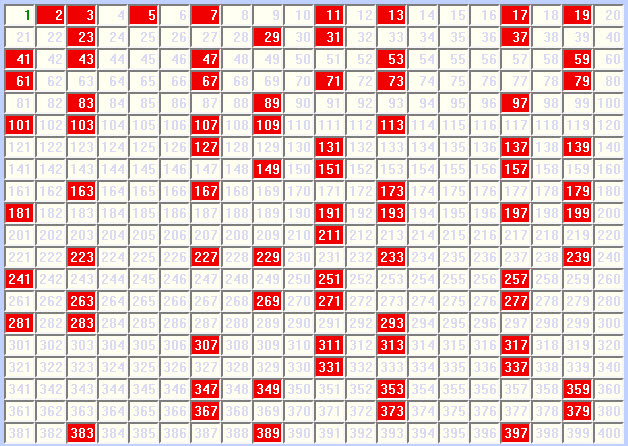
\includegraphics[width=\textwidth]{zeef.jpg}
\caption{Zeef van Eratosthenes}
\end{figure}

Om na te gaan of een groot geheel getal een priemgetal is, zijn er de laatste tientallen jaren verschillende nieuwe en moderne ‘zeven’ uitgevonden. Deze ‘zeven’ slagen er soms in getallen van honderden cijfers op te splitsen als een product van priemgetallen d.w.z. te ontbinden in priemfactoren. De meest bekende zeven zijn: de kwadratische zeef (Quadratic Sieve), de elliptische-kromme-methode (Elliptic Curve Method) en de getallenlichaam-zeef (Number Field Sieve). 

De kern van het kraken van RSA-codes schuilt in het ontbinden in priemfactoren van een zeer groot sleutelgetal m. Dit getal m, de modulus van de code, moet minstens tweehonderd cijfers bevatten om ‘praktisch’ onontbindbaar te zijn. Bij getallen van deze orde is de kans op een ontbinding binnen een aanvaardbare tijdspanne bijzonder klein. Hoe moeilijk het wel is om grote getallen in priemfactoren te ontbinden, willen we aantonen met ‘elliptische-krommen-methode’ die ook wel eens de ‘Lenstra-methode’ genoemd wordt, naar de Nederlandse wiskundige Hendrik Willem Lenstra Jr ($^{\circ}$ 1949). H. Lenstra, professor aan de universiteiten van Berkeley en van Leiden, ontdekte deze methode in het jaar 1985. Tot op heden is zijn algoritme het snelste algoritme voor ontbinding van een getal in priemfactoren met minder dan 50 cijfers. De krachtigste ontbinding met deze techniek tot hiertoe werd op 26 maart 2015 uitgevoerd door Ryan Propper. Hij vond een priemfactor van 64 cijfers uit het getal dat zelf 244 cijfers telt, nl $138^{59}+59^{138}$.

\begin{oef}
Ga naar de website http://www.alpertron.com.ar/ECM.HTM en bekijk de applet voor de ECM (elliptische-kromme-methode).

\begin{enumoef}
\item Ontbind $m= 402885473065764803780409750129828464897$ in factoren.
\item Hoeveel seconden heeft dit geduurd?
\item Hoeveel factoren heeft $m$?
\item In welk jaar is deze vraag ontworpen?
\item Open het programma Derive en ontbind opnieuw het getal $m$. Gebruik hiervoor de instructie factor(402885473065764803780409750129828464897).
\item Hoeveel minuten heeft dit geduurd?
\item Hoeveel tijd heb je nodig met de elliptische-kromme-methode om te bewijzen dat het Mersennegetal $2^{251}-1$ een priemgetal is?
\end{enumoef}
\end{oef}

\subsection{De totientfunctie van Euler (1707-1783)}

De getallen 10 en 21 zijn \emph{relatief priem}. Dit betekent dat ze geen gemeenschappelijke priemfactoren hebben. De priemfactoren van 10 zijn 2 en 5, de priemfactoren van 21 zijn 3 en 7. Een andere omschrijving voor \emph{relatief priem} is \emph{onderling ondeelbaar}.

Om te weten te komen hoeveel natuurlijke getallen kleiner dan 21 relatief priem zijn met 21 moet je deze getallen opsommen: 1, 2, 4, 5, 8, 10, 11, 13, 16, 17, 19 en 20. We tellen er 12. Leonard Euler was niet de eerste wiskundige die het verband tussen het getal $x$ en het hoeveelheid natuurlijke getallen kleiner dan $x$ en relatief priem met $x$ wist te appreciëren en te benutten. Wel gaf hij een naam aan deze hoeveelheid: de totient-functie. Wij spreken van de totient-functie van Euler. \emph{Totient} is de Latijnse vertaling van het woord \emph{hoeveelheid}. De totientfunctie wordt doorgaans genoteerd met de Griekse letter phi, bijvoorbeeld: $\varphi(21)=12$.

\begin{oef} Totientwaarden van kleine gehele getallen kunnen vaak nog manueel berekend worden door opsomming.

\begin{enumoef}
\item Som alle gehele getallen die kleiner zijn dan en relatief priem met 27. Hoeveel is $\varphi(27)$?
\item Som alle gehele getallen die kleiner zijn dan en relatief priem met 24. Hoeveel is $\varphi(24)$?
\end{enumoef}
\end{oef}

Voor grotere gehele getallen is deze opsomming arbeidsintensief. Ze kan ook vermeden worden, tenminste indien we over een formule voor de totient-functie beschikken. Deze formule is niet zo moeilijk op te stellen voor $x$-waarden die een macht zijn van een priemgetal.

\begin{oef} Stel het getal $x$ gelijk aan $5^4$ of aan 625.

\begin{enumoef}
\item Hoeveel gehele getallen kleiner dan $x$ zijn deelbaar door 5? 
\item Hoeveel gehele getallen kleiner dan $x$ zijn niet deelbaar door 5?
\item Bepaal $\varphi(x)$.
\item Zoek een formule voor $\varphi(p^n)$ met $p$ een priemgetal en $n$ een natuurlijk getal.
\end{enumoef}
\end{oef}

Totient-waarden van samengestelde getallen zijn iets moeilijker te berekenen. We onderzoeken nu de totient-waarde voor een product van twee machten van priemgetallen.

\begin{oef} Stel het getal $x$ gelijk aan $5^4 \cdot 7^3$.

\begin{enumoef}
\item Hoeveel gehele getallen kleiner dan $x$ zijn deelbaar door 5? 
\item Hoeveel gehele getallen kleiner dan $x$ zijn deelbaar door 7? 
\item Hoeveel gehele getallen kleiner dan $x$ zijn deelbaar door 5 en door 7? 
\item Hoeveel gehele getallen kleiner dan $x$ zijn niet deelbaar door 5 of 7? 
\item Gebruik de voorgaande resultaten om de waarde van $\varphi(x)$ te bepalen.
\item Zoek een formule voor $\varphi(p^n \cdot q^m)$ met $p$ en $q$ priemgetallen en $n$ een natuurlijk getal.
\item Ontbind deze formule in factoren en leer ze uit het hoofd.
\item Pas deze formule (of een veralgemening ervan) toe om de volgende waarden te berekenen: $\varphi(14641)$, $\varphi(2500)$,$\varphi(273)$,$\varphi(1225)$ en $\varphi(1232100)$.
\end{enumoef}
\end{oef}

\begin{figure} [h]
\label{vierentwintigpuntig}
\centering
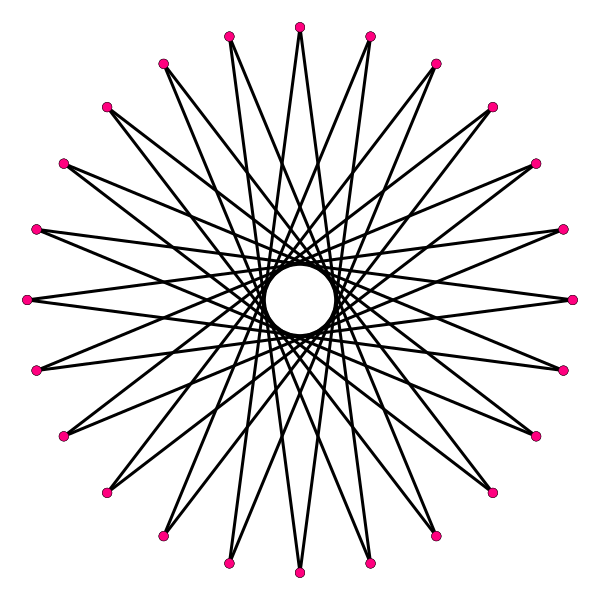
\includegraphics[width=0.5\textwidth]{24puntigester.png}
\caption{Een \{24/11\}-ster}
\end{figure}
  
Een eenvoudige toepassing op de totient-functie is het tellen van het aantal niet-gelijkvormige regelmatige $n$-puntige sterren. De volgende figuur toont een $\{24/11\}$-ster. Deze ster wordt genoteerd met de accoladenotatie van Schläfli. Het eerste getal in deze notatie, 24, staat voor het aantal punten van de ster. Het tweede getal, 11, staat voor de manier waarop de punten verbonden zijn. Bij deze ster is elk punt verbonden met zijn elfde opvolger. Op deze manier worden de hoekpunten verbonden met een veelhoekslijn die pas sluit nadat de 24 punten bezocht zijn.

Als je het getal 11 oordeelkundig vervangt, kan het zijn dat de veelhoekslijn zich opnieuw sluit na alle 24 punten bezocht te hebben. De ster zal dan scherpere of minder scherpe uitsteeksels hebben dan de $\{24/11\}$-ster. Echter, als je 11 vervangt door bijvoorbeeld 22 loopt het mis. De ster zal dan alleen de punten met een even rangnummer doorlopen en dat zijn er slechts 12.

\begin{oef}
Onderzoek hoeveel verschillende regelmatige 24-puntige sterren er bestaan.

\begin{enumoef}
\item Welke gehele waarden kan de parameter $k$ aannemen indien $\{24/k\}$ een 24-puntige sterveelhoek is?
\item Hoeveel verschillende sterren heb je dan als je twee sterren die congruent zijn maar een andere omloopszin hebben als één ster telt?
\item Hoeveel verschillende sterren heb je indien je de regelmatige 24-hoek niet langer als een ster beschouwt?
\item Wat is het verband tussen het aantal regelmatige 24-puntige sterren en $\varphi(24)$?
\item Wat is het verband tussen het aantal regelmatige $k$-puntige sterren en $\varphi(k)$?
\item Hoeveel niet congruente regelmatige 100-puntige sterren bestaan er?
\end{enumoef}
\end{oef}

\subsection{Het klokrekenen van Gauss (1777-1855)}

Bij kloklezen is het getal 15 gelijk aan het getal 3.  In principe zou je kunnen zeggen dat het getal 27 ook gelijk is aan het getal 3. Elk klokgetal is gelijk aan haar rest bij deling door 12. De wiskundige Gauss ontdekte dat voor vele toepassingen alleen de rest van een deling van belang was. Indien we de rest bij de deling door een geheel getal willen kennen dan doen we aan \emph{modulo-rekenen}. In moderne notatie noteren we modulo-gelijkheden als volgt:

\[27=3 \mod 12\]
\[100=9 \mod 13\]
\[1001=0 \mod 11\].

Bij modulo-rekenen mag je de modulo-bewerking naar believen toepassen op verschillende onderdelen van een formule. Dit maakt het voor de handrekenaar supereenvoudig om met kleine getallen te rekenen. Maar ook voor computers wordt het hierdoor een makkelijker om grote getallen te vermijden.

\begin{oef}
Reken de volgende waarden uit zonder gebruik te maken van digitale hulpmiddelen.

\begin{multicols} {2}
\begin{enumoef}
\item $2^{154} \mod 15$
\item $1001^{1002}+1003^{1004} \mod 10$
\item $36^{2017}+73^{2018} \mod 37$
\item $1302! \mod 1301$
\end{enumoef}
\end{multicols}
\end{oef}

\subsection{De kleine stelling van Fermat (1601-1665)}

Vele stellingen van Fermat zijn ontdekt als kanttekeningen in naslagwerken en brieven. De \emph{kleine stelling van Fermat} is gevonden in de kantlijn van een brief uit 1640. Deze stelling zegt dat voor elk getal $a$ kleiner dan en relatief priem met een modulus $m$ de onderstaande modulo-gelijkheid geldt.

\[a^{\varphi(m)}=1 \mod m\]

\noindent We laten het bewijs van de stelling achterwege. Het hoort eerder thuis in een cursus van \emph{groepentheorie}.

\begin{oef}
Reken de kleine stelling van Fermat na voor de volgende voorbeelden. Je mag hiervoor geen zakrekenmachine gebruiken.

\begin{multicols} {2}
\begin{enumoef}
\item $2^{\varphi(21)} \mod 21$
\item $5^{\varphi(24)} \mod 24$
\item $7^{\varphi(10)} \mod 10$
\item $3^{\varphi(25)} \mod 25$
\end{enumoef}
\end{multicols}
\end{oef}

\subsection{De stelling van Bézout (1730-1783) en Bachet (1581-1638)}

Deze twee wiskundigen die in een verschillende eeuw leefden, hebben hun naam gegeven aan dezelfde stelling. Claude Gaspard Bachet bewees ze in de zeventiende eeuw voor gehele getallen. Etienne Bézout bewees ze in de achttiende eeuw voor veeltermen. In deze cursus hebben we enkel de versie van Bachet nodig: Indien de getallen $e$ en $t$ relatief priem zijn, kunnen er steeds twee getallen $a$ en $b$ gevonden worden zo dat
\[a \cdot e + b \cdot t = 1.\]

Voor de getallen $e=14$ en $t=45$ vinden we bijvoorbeeld $a=-16$ en $b=5$ want $-16 \cdot 14 + 5 \cdot 45 =1$. Indien je gelukt hebt kan je de coëfficiënten $a$ en $b$ vinden door de veelvouden van $e$ en $t$ met je grafische zakrekenmachine in een tabel te zetten en beide tabellen te vergelijken. Indien een getal uit de eerste tabel slechts één eenheid verschilt van een getal uit de tweede tabel, heb je beet.

\begin{oef}
Test deze zoekactie uit met je grafische zakrekenmachine voor de volgende waarden van $e$ en $t$.

\begin{multicols} {2}
\begin{enumoef}
\item $e=14 \quad \textrm{en} \quad t=45$
\item $e=13 \quad \textrm{en} \quad t=45$
\item $e=19 \quad \textrm{en} \quad t=47$
\item $e=19 \quad \textrm{en} \quad t=17$
\end{enumoef}
\end{multicols}
\end{oef}

\subsection{Het delingsalgoritme van Euclides (ca 300 v.c.)}

Willen we de stelling van Bezout-Bachet narekenen voor grotere getallen dan moeten we de computer inschakelen. Bovendien moeten we gebruik maken van het inzicht van Euclides die bewees dat bij de deling van twee natuurlijke getallen de rest en het quotiënt uniek bepaald zijn.

We illustreren het algoritme van Euclides voor de getallen $t=8999$ en $e=997$. Vanaf nu nemen we aan dat $t$ groter is dan $e$. Door opeenvolgende delingen uit te voeren (zie hieronder), vinden we opeenvolgende resten $r_1=26$, $r_2=9$, $r_3=8$ en $r_4=1$. Deze resten zijn uniek bepaald. Ze zijn positief en ze vormen een strikt dalende rij. Het is dus logisch dat de laatste rest gelijk is aan 1.

\[ \left\{ \begin{aligned}
&8999&-&9\cdot997&=26 \\
&997&-&38\cdot26&=9 \\
&26&-&2\cdot9&=8 \\ 
&9&-&1\cdot8&=1
\end{aligned} \right.\qquad \Leftrightarrow \qquad
\left\{ \begin{aligned}
&t&-&9\cdot e &=r_1 \\
&e&-&38\cdot r_1 &=r_2 \\
&r_1&-&2\cdot r_2 &=r_3 \\ 
&r_2&-&1\cdot r_3 &=r_4
\end{aligned} \right.\]

In de onderstaande kader worden de opeenvolgende delingen uitgevoerd met het wiskundeprogramma Derive. Alle stappen van het programma worden verderop verklaard.

$\vspace{0.1cm}$
\begin{derive}
{Opeenvolgende delingen met algoritme van Euclides}
{\begin{align*}
\#1: \quad & \textrm{NotationDigits} := 60&&&&\\
\#2: \quad & \textrm{Precisiondigits}:= 60&&&&\\
\#3: \quad &t:=8999&&&&\\
\#4: \quad &e:=997&&&&\\
\#5: \quad & \textrm{quotientenrest}(x,y):=[\textrm{floor}(x,y),\textrm{mod}(x,y)]&&&&\\
\#6: \quad &\textrm{quotientenrest}(t,e)&&&&\\
\#7: \quad&&&&[9,26]&\\
\#8: \quad &\textrm{quotientenrest}(e,26)&&&&\\
\#9: \quad&&&&[38,9]&\\
\#10: \quad &\textrm{quotientenrest}(26,9)&&&&\\
\#11: \quad&&&&[2,8]&\\
\#12: \quad &\textrm{quotientenrest}(9,8)&&&&\\
\#13: \quad &&&&[1,1]&\\
\end{align*}}
\end{derive}
$\vspace{0.1cm}$

In stap \#1 en \#2 wordt de maximale getallengte vastgelegd op 60 cijfers. Getallen van deze lengte zullen later immers van belang zijn voor het codekraken. In stap \#3 en \#4 worden de getallen $t$ en $e$ gedefinieerd. Hiervoor gebruiken we het universele  toewijzingssymbool :=. In \#5 volgt een zelfgedefinieerde functie \emph{quotientenrest} die gehele getallen $x$ en $y$ als invoer heeft en een koppel van gehele getallen als uitvoer. De eerste component van de uitvoer is het gehele quotient van $x$ gedeeld door $y$. Om dit te berekenen wordt $x$ decimaal door $y$ gedeeld en wordt het antwoord naar beneden afgerond met de floor-functie. De tweede component is de rest van de deling van $x$ door $y$. Deze rest wordt berekend met de mod-functie. In de laatste vier stappen worden opeenvolgende quotiënten en resten opgevraagd. De antwoorden die aan de rechterkantlijn uitgelijnd zijn, worden automatisch berekend nadat er op de vereenvoudigingsknop gedrukt is.

Vervolgens keren we terug naar het bovenstaande stelsel. 

\[\left\{ \begin{aligned}
&t&-&9\cdot e &=r_1 \qquad (1)\\
&e&-&38\cdot r_1 &=r_2 \qquad (2)\\
&r_1&-&2\cdot r_2 &=r_3 \qquad (3)\\ 
&r_2&-&1\cdot r_3 &=r_4 \qquad (4)
\end{aligned} \right.\]

\noindent Als we vergelijking (1) invullen in (2) en (3), daarna (2) in (3) en (4) en tot slot (3) in (4) dan blijven alleen de letters $t$, $e$ en $r_4$ over. We kunnen manueel narekenen dat het verband tussen deze variabelen nu gegeven wordt door:

\[1038 \cdot e -115 \cdot t = r_4. \]

\noindent Vermits de laatste rest, $r_4$, gelijk was aan 1, hebben we op deze manier de betrekking van Bezout-Bachet gevonden. Om langdradige  substituties van vergelijkingen te vermijden, schakelen we ook nu Derive in.

$\vspace{0.1cm}$
\begin{derive}
{Berekening van coëfficiënten van Bezout-Bachet}
{\begin{align*}
\#14: \quad & t:= &&&&\\
\#15: \quad & e:= &&&&\\
\#16: \quad &r_1:=t-9\cdot e&&&&\\
\#17: \quad &r_2:=e-38\cdot r_1&&&&\\
\#18: \quad &r_3:=r_1-2\cdot r_2&&&&\\
\#19: \quad &r_4:=r_2-r_3&&&&\\
\#20: \quad &r_4&&&&\\
\#21: \quad &&&&1038\cdot e - 115 \cdot t&\\
\end{align*}}
\end{derive}
$\vspace{0.1cm}$

In de stappen \#14 en \#15 worden de variabelen $t$ en $e$ losgekoppeld van hun waarden. Mochten we dit vergeten dan zouden de letters $t$ en $e$ verderop bij de substituties vervangen worden door 8999 en 997. Hierdoor zou de lineaire combinatie van $t$ en $e$ waarnaar we op zoek waren, verdwijnen. De vier volgende stappen definiëren de resten $r_1$, $r_2$, $r_3$ en $r_4$. In deze definities worden de quotiënten 9, 28, 2 en 1 gebruikt. Die vonden we in de voorgaande Derivecode. In regel \#20 noteren we de laatste rest, $r_4$. Deze ultieme rest is altijd gelijk aan 1. Als we op de vereenvoudigingsknop drukken, worden er zoveel mogelijk substituties gedaan. De substituties van $t$ en $e$ door getallen zijn echter verijdeld. Daarom verschijnt er een lineaire combinatie van $t$ en $e$ in regel \#21 op het scherm. Deze combinatie is gelijk aan 1. Klaar, de lineaire combinatie van Bezout en Bachet is gekend.

\begin{oef}
Pas het algoritme van Euclides toe om de coëfficiënten van Bezout en Bachet te vinden voor de getallen $t$ en $e$ die onderling ondeelbaar zijn.

\begin{enumoef}
\begin{multicols} {2}
\item $t=1375 \quad \textrm{en} \quad e=1289$
\item $t=361 \quad \textrm{en} \quad e=343$
\item $t=501 \quad \textrm{en} \quad e=97$
\item $t=1843 \quad \textrm{en} \quad e=1001$
\item $t=2197 \quad \textrm{en} \quad e=1296$
\item $t=360 \quad \textrm{en} \quad e=343$
\end{multicols}
\end{enumoef}
\end{oef}


\begin{oef} Zoek de coëfficiënten van Bezout en Bachet voor de volgende waarden van $t$ en $e$.
\[t= 8 155 564 322 963 532 535 221 819 014 808 \quad \textrm{en} \quad e=100 003\]
\end{oef}
\newpage




\section{RSA-codes}
\subsection{Beschrijving van het mechanisme}

Bij eenvoudige coderingen kan uit het coderingsmechanisme vrij doorzichtig het decoderingsmechanisme afgeleid worden. Zo laat het coderingsmechanisme ‘schuif elke letter drie plaatsen door in het alfabet’ niets aan de verbeelding over. 

Bij RSA-codes is het verband tussen de twee mechanismen niet zo snel te achterhalen. RSA-systemen maken gebruik van een moeilijk in factoren te ontbinden modulus $m$. Deze modulus moet niet geheim gehouden worden. Buiten de ontwerper is er immers niemand die de ontbinding van $m$ kent of kan achterhalen. Verder wordt er gebruik gemaakt van twee exponenten: een openbare exponent $e$ die gebruikt wordt bij de codering en een geheime exponent $g$ die gebruikt wordt bij de decodering. Indien deze exponenten goed uitgedacht zijn, kan men elk getal $x$ kleiner dan $m$ coderen en decoderen door middel van machtsverheffing en modulo-rekenen. Dit zijn precies de bewerkingen waar computers van houden en waarvoor snelle algoritmen bestaan.

\subsubsection*{Coderingsmechanisme}

\smartdiagramset{back arrow disabled=true, set color list={magenta!50,blue!50,red!50}, border color = black, text color = black, module x sep = 4.4 cm, module minimum width = 3cm, text width = 3cm, font = \large, arrow line width = 3, arrow color = black, uniform arrow color = true, arrow style= latex-}
\smartdiagram[flow diagram:horizontal]{$x$, $x^e$, $x^e \textrm{ mod }m =y$}

\subsubsection*{Decoderingsmechanisme}

\smartdiagram[flow diagram:horizontal]{$y$, $y^g$, $y^g \textrm{ mod }m =x$}

$\vspace{0.1cm}$

Het moeilijkste onderdeel van het ontwerpen van RSA-codes is het op elkaar afstemmen van de getallen $m$, $e$ en $g$. Niet voor elke combinatie van deze getallen werkt de geschetste techniek. Goede getalwaarden zijn bijvoorbeeld  $m=403$, $e=343$ en $g=127$. We testen deze getallen uit door een bepaalde boodschap te coderen en het resultaat meteen opnieuw te decoderen. We kiezen hier voor de tekst \emph{abc} die via de alfabetische volgnummers omgezet wordt in het getal $x=123$.

\subsubsection*{Codering}

\smartdiagram[flow diagram:horizontal]{$123$, $123^{343}$, $123^{343} \textrm{ mod } 403 = 371$}

\subsubsection*{Decodering}

\smartdiagram[flow diagram:horizontal]{$371$, $371^{127}$, $371^{127} \textrm{ mod } 403 = 123$}

$\vspace{0.1cm}$


\subsection{Een spionage-opdracht}

\subsubsection*{De opdracht}
Een beroemde veldheer zendt een Engelstalig bericht door van twee zinnen. Deze zinnen worden omgezet in de getallen $x_1$ en $x_2$ door elke letter te vervangen door zijn volgnummer in het alfabet.

\begin{figure} [h]
\label{alfabet}
\centering
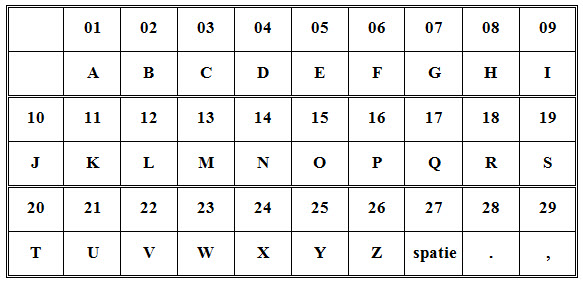
\includegraphics[width=\textwidth]{alfabet.jpg}
\caption{Omzettingstabel van letters naar cijfers}
\end{figure}

\noindent De codering gebeurt aan de hand van de volgende openbare gegevens:

\[
\begin{aligned}
&m=8 155 564 322 963 545 435 233 042 348 043\\
&e=100 003.\\
\end{aligned}
\]

\noindent De doorgeseinde berichten worden echter onderschept door een spion:

\[
\begin{aligned}
&y_1=701 056 613 179 062 784 283 291 508 801\\
&y_2=6 001 020 772 977 398 118 504 479 017 163.\\
\end{aligned}
\]

\noindent Zonder de geheime exponent kan de spion niet veel uit deze getallen opmaken. Daarom probeert hij met geduld de geheime exponent te achterhalen. Jij moet hem hierbij helpen.

\subsubsection*{Methode om een RSA-code te kraken}
Probeer eerst de openbare modulus $m$ te ontbinden in twee priemfactoren: $p$ en $q$. Je kan dit doen door het wiskundeprogramma Derive aan het rekenen te zetten. Heb je een aftandse computer dan kan dit meer dan een half uur in beslag nemen. Maar met een moderne rekenprocessor kost het je hooguit een kwartier … een verwaarloosbare beproeving voor de modale RSA-kraker. Als alles goed gaat, merk je dat twee priemfactoren elk een respectabele omvang hebben.

\[m=p \cdot q\]

In de tweede stap berekenen we hoeveel getallen kleiner dan de modulus $m$ en relatief priem zijn met $m$. Dit getal $t$ is de totient-waarde van de modulus $m$. Omdat $m$ een product is van twee priemgetallen (met exponent 1) is het niet zo moeilijk om deze totient-waarde te berekenen.

\[t=\varphi(m)=(p-1)p^0 \cdot (q-1)q^0=(p-1)(q-1)\]

Bij correcte RSA-codes, zoals deze, blijken de getallen $t$ en $e$ onderling ondeelbaar te zijn. Met de gekende getallen $t$ en $e$ kan je het algoritme van Euclides toepassen en kan je de coëfficiënten $a$ en $b$ bepalen waarvoor:

\[a \cdot e = b \cdot t = 1.\]

De coëfficiënt $a$ bij de openbare exponent $e$ komt nu overeen met de geheime exponent $g$. Waarschijnlijk schrik je nu wel even van de waarde van de geheime exponent $g$. Dit getal is beduidend groter dan de openbare exponent $e$. Dat is ook de bedoeling. Geheime berichten schrijven hoeft niet echt moeilijk te zijn: het getal $e$ is tamelijk kort. Geheime berichten ontcijferen mag best ingewikkeld zijn: het getal $g$ is eerder lang.

\[g=a\]

Nu kan het decoderen van de geheime boodschap beginnen. Je kent de modulus $m$ en de geheime exponent $g$ … dit is voldoende om je spionagewerk te voltooien. 

\subsubsection*{Verwerking met Derive}

Om vlot te coderen en te decoderen in Derive is het nuttig een file aan te maken. We laten hem in deeltjes zien. Een eerste deel bevat alle gegevens.

$\vspace{0.1cm}$
\begin{derive}
{Een spionage-opdracht}
{\begin{align*}
\#1: \quad & \textrm{NotationDigits} := 60&&&&\\
\#2: \quad & \textrm{Precisiondigits}:= 60&&&&\\
\#3: \quad &m:= 8 155 564 322 963 545 435 233 042 348 043&&&&\\
\#4: \quad &e:=100003&&&&\\
\#5: \quad &y_1:=701 056 613 179 062 784 283 291 508 801&&&&\\
\#6: \quad &y_2:=6 001 020 772 977 398 118 504 479 017 163&&&&\\
\end{align*}}
\end{derive}
$\vspace{0.1cm}$

In een tweede deel ontbinden we de modulus in factoren en bereken de totientfunctie van deze modulus. Om niet alles te verklappen, hebben we sommige getallen in de derivecode verminkt door de staarten te vervangen door stippeltjes. Hierdoor lijken de getallen $m$ en $t$ er hetzelfde uit te zien maar in werkelijkheid zijn ze verschillend.
 
$\vspace{0.1cm}$
\begin{derive}
{Een spionage-opdracht}
{\begin{align*}
\#7: \quad & \textrm{factor} (m) &&&&\\
\#8: \quad &&&&666666777777727 \cdot 1223334444\dots&\\
\#9: \quad &p:= 666666777777727&&&&\\
\#10: \quad &q:=1223334444\dots &&&&\\
\#11: \quad &t:=(p-1)(q-1)&&&&\\
\#12: \quad &&&&81555643229635325\dots&\\
\end{align*}}
\end{derive}
$\vspace{0.1cm}$

De waarden van $t$ en $e$ zijn nu gekend. Deze getallen zijn relatief priem. In een derde deel van het derivebestand voeren we opeenvolgende delingen uit van $t$ en $e$ volgens het algoritme van Euclides. We gaan hiermee door tot we 1 als rest vinden. Ook in deze schermafdruk hebben we getallen gecamoufleerd door enkel de eerste cijfers te vermelden. Als alles goed uitgevoerd wordt, heb je tien euclidische delingen nodig om tot de uiteindelijke rest van 1 te komen.

$\vspace{0.1cm}$
\begin{derive}
{Een spionage-opdracht}
{\begin{align*}
\#13: \quad & \textrm{quotientenrest}(x,y):=[\textrm{floor}(x,y),\textrm{mod}(x,y)]&&&&\\
\#14: \quad &\textrm{quotientenrest}(t,e)&&&&\\
\#15: \quad&&&&[815\dots, 538\dots]&\\
\#16: \quad &\textrm{quotientenrest}(e,538 \dots)&&&&\\
\#17: \quad&&&&[1, 461\dots]&\\
\#18: \quad &\textrm{quotientenrest}(538 \dots, 461 \dots)&&&&\\
\#19: \quad&&&&[1, 778\dots]&\\
\end{align*} \textrm{enzovoort \dots} }
\end{derive}
$\vspace{0.1cm}$

Nu kunnen de variabelen $t$ en $e$ losgekoppeld worden en kunnen de parameters $a$ en $b$ uit de stelling van Bezout en Bachet berekend worden. Zoals we eerder getoond hebben, moeten er opeenvolgende resten $r_1, r_2, r_3, \dots, r_{10}$ gedefinieerd worden. Derive zal deze resten handig in elkaar substitueren zo dat er slechts drie onbekenden overblijven: $t$, $e$ en $r_{10}$. Deze betrekking is de formule van Bezout en Bachet. Je ziet ze in gecamoufleerde versie onderaan het volgende derivebestand.

$\vspace{0.1cm}$
\begin{derive}
{Een spionage-opdracht}
{\begin{align*}
\#34: \quad & t:=&&&&\\
\#35: \quad & e:=&&&&\\
\#36: \quad & r_1:=t-815\dots e &&&&\\
\#37: \quad & r_2:= e-r_1&&&&\\
\#38: \quad & r_3:= r_1-r_2&&&&\\
\#39: \quad & r_4:= r_2-5r_3&&&&\\
&\textrm{enzovoort \dots}&&&&\\
\#46: \quad & r_4&&&&\\
\#47: \quad &&&& 762\dots e - 9354 t&\\
\end{align*} }
\end{derive}
$\vspace{0.1cm}$

De coëfficiënt bij de openbare exponent $e$ is de geheime exponent $g$. In een volgend deeltje van de derivecode schrijven we enkele programmalijnen die het coderen en decoderen vereenvoudigen. We mogen echter niet vergeten de openbare exponent $e$ opnieuw een waarde te geven.

$\vspace{0.1cm}$
\begin{derive}
{Een spionage-opdracht}
{\begin{align*}
\#48: \quad & g:=762\dots&&&&\\
\#49: \quad & e:=100003&&&&\\
\#50: \quad & \textrm{codeer}(x):=\textrm{mod}(x^e,m) &&&&\\
\#51: \quad & \textrm{decodeer}(x):=\textrm{mod}(x^g,m) &&&&\\
\end{align*} }
\end{derive}
$\vspace{0.1cm}$

Alles is nu in gereedheid gebracht voor de ontknoping. We decoderen de geheime getallen $y_1$ en $y_2$ en maken de proef door de gevonden getallen $x_1$ en $x_2$  opnieuw te coderen. Indien we de onderschepte getallen $y_1$ en $y_2$ terugvinden dan mag heel de kraakoperatie als geslaagd beschouwd worden. 

Er is nog een kleine complicatie waar we de aandacht willen op vestigen: nullen aan het begin van een getal vallen altijd weg. Als een zin bijvoorbeeld met de letter \emph{b} begint dan zal het overeenkomstige alfabetische volgnummer 02 automatisch vervangen worden door 2, waardoor er misverstanden kunnen ontstaan bij het groeperen van van de boodschap in blokjes van twee cijfers. Daarom is het raadzaam een zin te beginnen met bijvoorbeeld een spatie, die in deze oefening overeenkomt met volgnummer 27.

$\vspace{0.1cm}$
\begin{derive}
{Een spionage-opdracht}
{\begin{align*}
\#52: \quad & \textrm{decodeer}(y_1)&&&&\\
\#53: \quad &&&&270102\dots&\\
\#52: \quad & \textrm{decodeer}(y_2)\dots&&&&\\
\#53: \quad &&&&270518\dots&\\
\#54: \quad & x_1:=270112\dots&&&&\\
\#55: \quad & x_2:=270518\dots&&&&\\
\#52: \quad & \textrm{codeer}(x_1)&&&&\\
\#53: \quad &&&&701056\dots&\\
\#52: \quad & \textrm{codeer}(x_2)\dots&&&&\\
\#53: \quad &&&&600102\dots&\\
\end{align*} }
\end{derive}
$\vspace{0.1cm}$

\begin{oef}
Voer al deze programmaregels in via het programma Derive en vereenvoudig de uitdrukkingen waar nodig.

\begin{enumoef}
\item Mag je deze codekraking als geslaagd beschouwen?
\item Vertaal $x_1$ en $x_2$ in letters. Welke Engels palindroom werd er onderschept.
\item Vertaal de tekst. Let op: het middelste woord is Oudengels.
\item Wie zou deze tekst uitgesproken kunnen hebben? Verklaar in welke context hij dit deed.
\item Waar kwam deze veldheer aan zijn einde? Waar ligt hij nu begraven?
\item Is deze palindroom \emph{volmaakt}, m.a.w. zijn ook de spaties spiegelsymmetrisch ten opzichte van het midden van de zin?
\end{enumoef}
\end{oef}

\subsection{Bewijs van het mechanisme}

Om helemaal overtuigd te raken van de werking van de RSA-codes is het belangrijk aan te tonen dat het decoderingsmechanisme ($x=y^g \textrm{ mod } m$) volgt uit het coderingsmechanisme ($y=x^e\textrm{ mod } m$) en omgekeerd.

\begin{oef}
Hieronder wordt de equivalentie van het coderingsmechanisme en het decoderingsmechanisme aangetoond. Verklaar elke stap.
\end{oef}

\begin{proof}
\begin{align*}
& y=x^e \textrm{ mod }m&&\textrm{coderingsmechanisme}\\
\Leftrightarrow \qquad & y^g=(x^e)^g \textrm{ mod }m&&\dots\\
\Leftrightarrow \qquad & y^g=x^{g \cdot e} \textrm{ mod }m&&\dots\\
\Leftrightarrow \qquad & y^g=x^{a \cdot e} \textrm{ mod }m&&\dots\\
\Leftrightarrow \qquad & y^g=x^{1-b \cdot t} \textrm{ mod }m&&\dots\\
\Leftrightarrow \qquad & y^g=x\cdot (x^t)^{-b} \textrm{ mod }m&&\dots\\
\Leftrightarrow \qquad & y^g=x\cdot (x^{\varphi(m)})^{-b} \textrm{ mod }m&&\dots\\
\Leftrightarrow \qquad & y^g=x\cdot 1^{-b} \textrm{ mod }m&&\dots\\
\Leftrightarrow \qquad & y^g=x\textrm{ mod }m&&\textrm{decoderingsmechanisme}\\
\end{align*}
\end{proof}


\subsection{Een tweede spionage-opdracht}

Een tweede onderschept bericht komt van een politieker met een ambitieus plan, dat een economische heropleving aan zijn land zou moeten geven. Deze geromantiseerde uitspraak is, net als die uit de vorige spionage-opdracht, niet autenthiek. Ze werd voor de eerste keer vermeld in 1948 en is sindsdien zo vaak geciteerd dat ze een historische allure kreeg. 

De openbare modulus van de geheimcode en de openbare exponent zijn:

\[
\begin{aligned}
&m:=40469413478001783496373983733007377\\
&e:= 11951.\\
\end{aligned}
\]

\noindent Het onderschepte bericht bestaat uit drie delen:

\[
\begin{aligned}
&y_1= 3670025767580870203930440385693528\\
&y_2= 28750768500525900747770181901972524\\
&y3= 15577635291675694201520438341616192.\\
\end{aligned}
\]

\noindent Er werd gebruik gemaakt van het volgende alfabetische overzicht van letters en leestekens.

\begin{figure} [h]
\label{alfabet2}
\centering
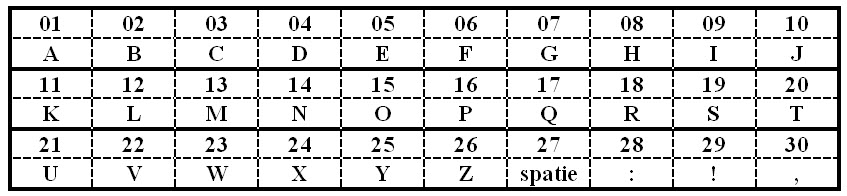
\includegraphics[width=\textwidth]{alfabet2.jpg}
\caption{Alfabetisch register}
\end{figure}

Normaalgezien is deze boodschap niet te decoderen zonder de geheime exponent $g$. Omdat de modulus in dit voorbeeld slechts 35 cijfers telt, is het voor de meeste rekenprogramma's wel haalbaar $m$ binnen een redelijke tijd in factoren te ontbinden. Op deze manier kan de geheime exponent op sluwe wijze achterhaald worden. Veiliger zou het geweest zijn wanneer de modules $m$ 70 of meer cijfers zou tellen.

\begin{oef}
Decodeer de geheime boodschap met een derivebestand.

\begin{enumoef}
\item Vertaal dit bericht. 
\item In welk jaar en in welke context zou een politieker deze uitspraak  kunnen hebben gedaan? 
\item Welke speciale speciale acties werden er in 2015 ondernomen om de historische doorbraak, waar deze uitspraak naar verwijst, te herdenken?
\item Welke taalkundig stijlkenmerk maakt deze uitspraak zo fascinerend (rijmpatroon, alliteratie, woordspeling, chiasme, palindroom, volmaakte palindroom, pleonasme, polysyndeton, \dots)?
\end{enumoef}
\end{oef}

\newpage


\section{Codekraken in Sage}
\subsection{Sage en SageMathCloud}
Doorheen het vorige hoofdstuk zal duidelijk geworden zijn dat codekraken een activiteit is die moet toevertrouwd worden aan de zwaardere wiskundesoftware. We zouden beroep kunnen doen op gerenommeerde, betalende wiskundepakketten als Maple, Mathematica of Matlab. Maar die vragen een flinke financiële bijdrage van de gebruiker. Vandaar dat onze keuze voor dit project uitgaat naar Sage, momenteel een van de krachtigste opensourcepakketten voor wiskundige toepassingen. Sage werd ontwikkeld door William Stein aan de Universiteit van Washington. Sinds het voor de eerste maal op het internet kwam, februari 2005, tot halverwege 2016 werd alle software ontwikkeld door vrijwilligers. Nu zijn er ook betaalde programmeurs achter de schermen aan het werk. Sage geniet elk jaar meer bijval bij wetenschappers die zich afzetten tegen de commerciële aspecten van computergebruik. Sinds enkele jaren wordt Sage ook gepromoot en aangeleerd aan de UGent.

Sage is sterk in om het even welke tak van de wiskunde: algebra, combinatoriek, analyse, getaltheorie, groepentheorie en vectorruimten, \dots Bovendien is er een  grafische ondersteuning voor 2D-plots, 3D-plots, histogrammen, niveaulijnendiagrammen, \dots die niet moet onderdoen voor de grafische functionaliteit van commerciële software. Buiten de klassieke wiskundige toepassingen zijn er in Sage ook minder verwachte applicaties uitgewerkt. Kan je bijvoorbeeld een bepaalde hardnekkige sudoku niet oplossen, vraag het dan maar aan Sage. Die weet er raad mee.

\subsubsection*{Voordelen van Sage}

Sage beschikt over snelle en krachtige algoritmen. Het steunt hierbij op verschillende andere pakketten zoals Maxima en het gebruikt een taal die verwant is met Python. Een getal van 30 cijfers ontbinden in een product van twee priemgetallen van 15 cijfers duurt slechts enkele seconden, dit in tegenstelling met de ontbinding in Derive. Om de veiligheid van een RSA-code te garanderen moeten de priemfactoren vanaf nu minstens de dubbele lengte krijgen.

In Sage zijn er ook veel meer algoritmen voorgeprogammeerd dan in Derive. Je kan de coëfficiënten van het algoritme van Bezout bijvoorbeeld met één enkel commando berekenen. Ook bestaat er een instructie powermod die de modulorest berekent van een macht van een geheel getal. Dit is precies de kern van de RSA-versleuteling.

Sinds korte tijd bestaat er een manier om Sagebestanden in de cloud te bewaren en om er met verschillende auteurs tegelijkertijd aan te werken. Deze voordelen worden geboden door SageMathCloud, ook weer freeware. Je kan hiervoor intekenen op de website https://cloud.sagemath.com. 

\begin{figure} [h]
\label{sagelogo}
\centering
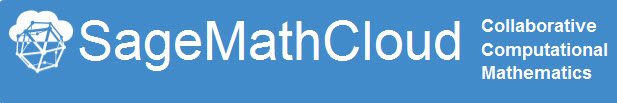
\includegraphics[width=\textwidth]{sagelogo.jpg}
\caption{Logo van SageMathCloud}
\end{figure}

\subsubsection*{Doelstellingen}

Wellicht vraag je je af waarom we, na de programmering in Derive, alles nog een keertje moeten overdoen in Sage. Een eerste reden is duidelijk: door zijn rekenkracht is Sage bijzonder geschikt voor codekraken. In vergelijking hiermee is Derive een speelgoedprogramma, dat evenwel geschikter is voor didactische doeleinden. Vandaar ook dat we de theorie eerst opgebouwd hebben met Derive.

Software evolueert hoe langer hoe sneller. Wat vandaag in de mode is, is volgend jaar voorbijgestreefd. Het is dan ook belangrijk om snel nieuwe software te kunnen doorgronden. Zelfs al heb je weinig of geen voorkennis, je moet je altijd uit de slag kunnen trekken met online handleidingen en door het snuffelen op discussieforums. Professionele programmeurs werken meestal op een dubbel scherm, eentje om te schrijven en eentje om opzoekingen te doen.

Een derde doelstelling van dit project is het leesbaar kunnen presenteren van een programma. Dit doe je uiteraard door genoeg bindteksten tussen de programmaregels op te nemen. Als je formules in de bindteksten opneemt, moet je er wel op letten dat je hiervoor de gepaste codes kent. Sage ondersteunt \LaTeX-codes. \LaTeX is wereldwijd het populairste formaat om wetenschappelijke teksten te editeren. Ook deze handleiding is gezet in \LaTeX. De opmaak onderscheidt zich door haar strakheid sterk van die van Word. Binnen elke Sage-werkmap kan je aparte verslagen toevoegen in \LaTeX. Schrijven in \LaTeX \,is een kunst op zich waar je stapje voor stapje moet inkomen.

\subsection{Een spionage-opdracht in Sage}

We hernemen hier de eerste spionage-opdracht uit hoofdstuk 3. Het is de bedoeling ze te herprogrammeren met een minimum aan aanwijzingen en een maximum aan doorzettingsvermogen en zelfredzaamheid. Op de figuur hieronder zie je een deeltje van een mogelijk  eindresultaat. In het Sage-bestand hieronder wisselen teksten af met kleine blokjes formules. Door het programma op deze manier in te delen, kan je makkelijker fouten detecteren en verbeteren.

\begin{figure} [h]
\label{sagescreenshot}
\centering
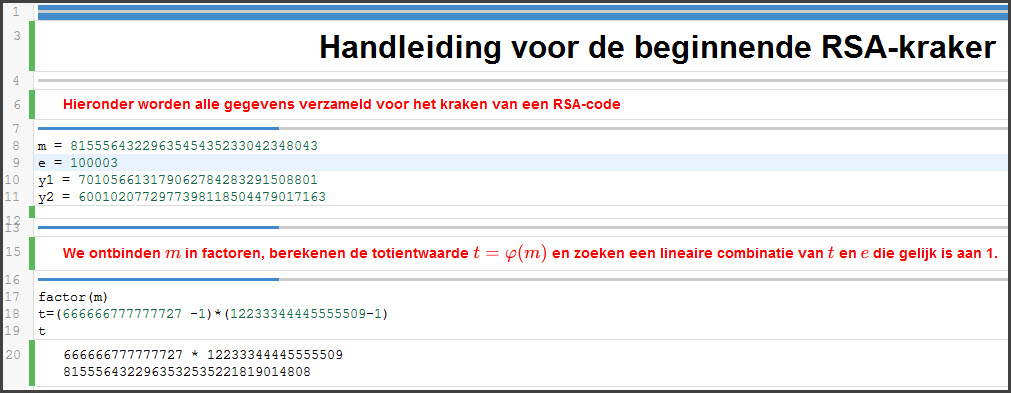
\includegraphics[width=1.3\textwidth]{Sage.jpg}
\caption{Screenshot RSA-bestand in Sage}
\end{figure}

\subsubsection*{Een account aanmaken en een nieuw bestand openen}

Voor je kan werken in SageMathCloud (surf naar https://cloud.sagemath.com) moet je een account aanmaken waarop je moet inloggen. Als dit gelukt is maak je een nieuw project aan via de optie \emph{Create a new project}. Noem dit project \emph{RSA-codes}. Als je binnen dit project naar \emph{Settings en configurations} gaat kan je eventueel kiezen wie er \emph{collaborator} of medewerker is. Vul het mailadres in van de medewerkers (of van de leerkracht die je werk moet verbeteren). Medewerkers krijgen automatisch inzage in je programma. Meer nog, ze kunnen er simultaan met jou aan werken. 

Binnen een project kan je verschillende files creëren. Je hebt de keuze tussen een tiental verschillende typen. De belangrijkste zijn: een sageworksheet en een \LaTeX -bestand. Maak nu een sageworksheet aan met de knop \emph{Create}. Geef het de naam \emph{Spionage-opdracht}

\subsubsection*{Teksten invoeren}

Meteen verschijnt er een blanco invoerblad op je computerscherm. Dit blad moet je vullen met formules en teksten. Telkens als je een formule of een tekst hebt ingevoerd, kan je deze evalueren door op de knop \emph{Run} te drukken. Een lichtblauw knipperend streepje boven de formule geeft dan aan dat Sage aan het denken (lees: evalueren) is. Wanneer het knipperen stopt, verschijnt het antwoord op je vraag of verschijnt er een foutmelding. In het laatste geval moet je een correctie aanbrengen en moet je opnieuw \emph{Runnen}.

Voor je met de wiskundige programmaregels begint, is het best enkele titeltjes en verklarende teksten klaar te zetten. Zo blijft je programma leesbaar voor anderen. Een tekst begint altijd met  \emph{\%html} waarna de tekst volgt. Hoe je de teksten verder opmaakt (vetten, kleuren, centreren \dots), kan je zelf op het internet opzoeken. 

Als je in je verklarende teksten wiskundige variabelen of wiskundige formules wil opnemen dan zet je die steeds tussen dollartekens. Dit is typisch voor \LaTeX. Een andere kenmerk van \LaTeX \, is dat elke wiskundige term voorafgegaan wordt van een backslash. Zo weet de compiler \LaTeX \,dat de term niet per se letterlijk moet weergegeven worden maar dat hij moet vertaald worden met een specifiek symbool.

Hieronder zie je drie formules die in een tekst opgenomen kunnen worden. Probeer de notatie te begrijpen: de eerste formule is de stelling van Pythagoras, de tweede is de verdubbelingsformule van de cosinus en de derde is een van de oplossingen van een vierkantsvergelijking.

\begin{minipage}{\textwidth}
\vspace{2 mm}
\begin{verbatim}
$\sqrt{a^2+b^2}=c$
$\cos (2 \cdot \alpha)= 1 - 2 \cos^2 \alpha$
$x_1=\frac{-b+\sqrt{D}}{2a}$
\end{verbatim}
\vspace{2 mm}
\end{minipage} 

\noindent Na het \emph{Runnen} zien de formules er als volgt uit:

\vspace{2 mm}
\begin{tabular}{lllll}
$\sqrt{a^2+b^2}=c$ &&&&\\
$\cos (2 \cdot \alpha)= 1 - 2 \cos^2 \alpha$ &&&&\\
$x_1=\frac{-b+\sqrt{D}}{2a}$ &&&&\\
\end{tabular}
\vspace{2 mm}

\subsubsection*{Het kraakprogramma}

In een eerste programmablok zou je alle gegevens kunnen toewijzen aan symbolen: de modulus $m$, de openbare exponent $e$ en de onderschepte berichten $y_1$ en $y_2$. Let op: het toewijzingsteken is in Sage een gewoon gelijkheidsteken.

Het tweede gedeelte van het kraakprogramma bevat de ontbinding in factoren van $m$ en de berekening van de totientwaarde $t=\varphi(m)$. Het zal je niet ontgaan dat het ontbinden in factoren onnoemelijk veel vlugger gaat dan in Derive.

In een derde onderdeel van het programma berekenen we de lineaire combinatie van $t$ en $e$ die gelijk is aan 1. Ditmaal lukt het zonder de ketting van opeenvolgende delingen. Er bestaat immers een instructie \emph{xgcd}. Zoek maar op hoe deze instructie werkt. Ze levert je de geheime exponent $g$ op.

Definieer vervolgens een functie om te coderen en te decoderen. Op het internet vind je handige  informatie over functiedefinities in Sage. Decodeer hiermee het onderschepte bericht en maak de proef door opnieuw te coderen. Dit is het vierde deel van je programma. Hierna zou je kunnen stoppen.

Maar als je echt het onderste uit de kan wil, dan schrijf je nog een vijfde blokje programmacode, waarin je het gedecodeerde bericht in getalvorm automatisch laat omzetten in een gedecodeerd bericht in lettervorm. Wellicht moet je voor dit deel erg veel opzoekwerk doen en neemt dit zoekwerk meerdere dagen in beslag.

Ik doe een suggestie. Je zou de gedecodeerde berichten $x_1$ en $x_2$ kunnen omzetten in een lijst van getallen met twee cijfers. De letters van het alfabet uit de omzettingstabel kan je in een andere lijst zetten. Door deze lijsten met elkaar in verband te brengen, kan je een lijst maken met de opeenvolgende letters (en leestekens) van het bericht. Mocht je deze lijst nog kunnen omzetten in een \emph{woord} of in een \emph{zin} dan was het kraakprogramma perfect.



\subsection{Een straffere spionage-opdracht in Sage}

Een wiskundeleerkracht van Edugo schrijft een geheime mail naar zijn directeur. Om deze mail te beveiligen tegen inmenging van nieuwsgierige leerlingen werd hij met een krachtige RSA-sleutel gecodeerd. Een modulus $m$ van 75 cijfers leek hiervoor voldoende veilig. De openbare gegevens van de RSA-code zijn:

\[
\begin{aligned}
&m=202783501414149470878532022214791138076579405702371707086574775134770297207\\
&e=100000007.\\
\end{aligned}
\]
 \noindent Zoals altijd wordt er een alfabetisch register gebruikt om letters om te zetten in cijfers en omgekeerd. Deze omzettingstabel hoeft natuurlijk niet verborgen te blijven. De leerkracht gebruikte het register uit figuur 8. Het verschilt slechts weinig van de eerder gebruikte registers.
 
\begin{figure} [h]
\label{alfabet2}
\centering
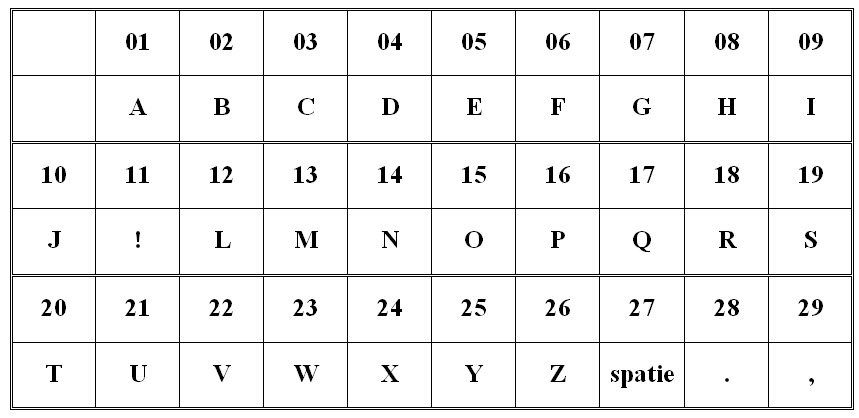
\includegraphics[width=\textwidth]{alfabet3.jpg}
\caption{Alfabetisch register}
\end{figure}

Jij hebt het bericht aan de directeur op slinkse wijze onderschept. Het bestaat uit zes woorden. Als je deze woorden kan decoderen is je missie geslaagd. Schrijf een Sage-programma waarin dit onderschepte bericht gedecodeerd wordt en los de opdracht in de geheime boodschap op.

\[
\begin{aligned}
&x_1=91107399053297051423384464760464671588858993154572075501499828940722910637\\
&x_2=79523414152366341862866174751492360839039481777822124889597473168578629610\\
&x_3=101943657700410929557586519483461382000937421060250687718605122239934544839\\
&x_4=84011139702996907082520918770400242972308793148096752027183505368856605775\\
&x_5=174523304627798124281115308933809841037046034044795772895654815277112696944\\
&x_6=194484576345447805211705420086897747753497008610556597940574009488195795276\\
\end{aligned}
\]


\pagebreak
\tableofcontents

\end{document}